\section{历史视角}

“无论你把对称的含义定义得多么宽泛或狭窄，它都是人类自古以来试图理解并创造秩序、美与完美所凭借的一种观念。”\marginnote{
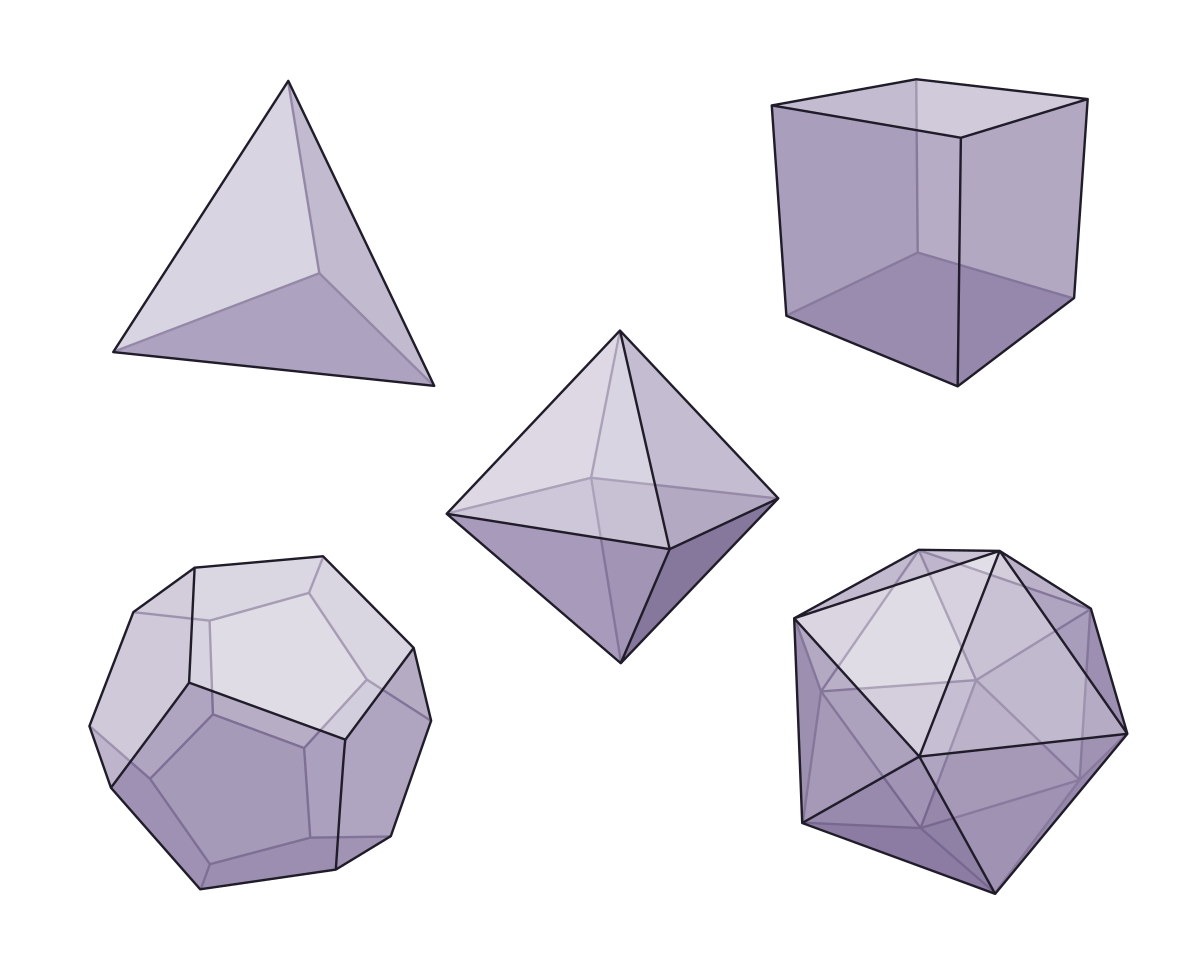
\includegraphics[width=0.9\linewidth]{figures/platonic_solids.png}
四面体、立方体、八面体、十二面体和二十面体称为\emph{Platonic 立体}。}
%
这个略带诗意的对称定义，出自伟大数学家 Hermann \citet{weyl2015symmetry} 的同名著作；那是他从 Princeton Institute for Advanced Study 退休前夕的\emph{绝唱}。
%
Weyl 追溯了对称自古以来在科学与艺术中的特殊地位，从 Sumerian 的对称设计，到因圆具有旋转对称性而认为它是完美形状的 Pythagoreans。
%
Plato 认为，今天以他命名的五种正多面体具有如此基础的地位，以至于它们必定是塑造物质世界的基本构件。
%
不过，尽管人们认为 Plato 创造了术语 \textgreek{summetr'ia}（字面意为“相同的尺度”），他只是含糊地用它表达艺术中比例之美与音乐中的和谐。
%
天文学家兼数学家 Johannes Kepler 首次尝试对水晶体的对称形状作严格分析。在他的论著《六角雪花》中，\marginnote{
%\includegraphics[width=0.9\linewidth]{figures/de_nive.png}
其完整书名为
\emph{Strena, Seu De Nive Sexangula}（“新年礼物，或论六角雪花”）；正如标题所暗示的，这是 Kepler 于 1611 年作为圣诞礼物寄给资助者兼友人 Johannes Matthäus Wackher von Wackenfels 的一本小册子。}他把雪花的六重二面体结构归因于粒子的六角密堆积；尽管这一观念早于人们对物质形成方式的清晰认识，却至今仍是晶体学的基础 \citep{ball2011retrospect}。




%D'Arcy Thompson {\em On Growth and Form} appeals to the notions of symmetry to explain the structure of biological life forms. 

\paragraph{数学与物理学中的对称性}
在现代数学中，对称性几乎毫无例外地用群论语言表达。%
这一理论的起源通常归功于 {\'E}variste Galois；他创造了这个术语，并在 19 世纪 30 年代用它研究多项式方程的可解性。
%
另外两个与群论相关的名字是 Sophus Lie 和 Felix Klein；二人曾经相识，并在一段时期内开展了富有成效的合作 \citep{tobies2019felix}。前者后来发展了今天以其名字命名的连续对称性理论；后者则在本文开头提到的 Erlangen Programme 中宣称群论是组织几何学的原则。Riemann 几何被明确排除在 Klein 的统一几何图景之外，直到五十年后才被纳入其中，这在很大程度上得益于 {\'E}lie Cartan 在 20 世纪 20 年代的工作。

%unified multiple geometries. 

%Physics:  


Klein 在 G\"ottingen 的同事 Emmy Noether 证明，物理系统作用的每一种可微对称性都有相应的守恒律 \citep{variationsprobleme1918nachr}。这在物理学中是一项惊人的结果：在此之前，发现能量守恒等基本定律需要细致的实验观测，即便如此，得到的也只是没有理论来源的经验结果。Noether 定理——用诺贝尔奖得主 Frank Wilczek 的话说，是“20 与 21 世纪物理学的指路明星”——表明能量守恒源于时间的平移对称性。这一观念相当直观：实验结果不应取决于实验是在今天还是明天进行。

%That theorem has been a guiding star to 20th and 21st century physics,” says theoretical physicist Frank Wilczek


%[FROM WIKI]
与电荷守恒相关的对称性，是电磁场的全局\emph{规范不变性}；\marginnote{Weyl 于 1919 年首次提出一个后来证明不正确的猜想：尺度或“规范”变化下的不变性是电磁学的一种局部对称性。术语 \emph{gauge}（德语为 \emph{Eich}）是类比铁路的不同轨距而选定的。%Although Weyl's choice of the gauge was initially incorrect, the name ``gauge'' stuck to the approach, and
量子力学发展之后，\cite{weyl1929elektron} 用波相位变化取代尺度因子，修正了规范的选择。见 \cite{straumann1996early}。
}它最早出现在 Maxwell 对电动力学的表述中 \citep{maxwell1865viii}；%This symmetry is related to the fact that the electric and magnetic fields are not changed by different choices of the value representing the zero point of electrostatic potential;
然而，其重要性最初并未受到注意。% in the earliest formulations.
%
%Similarly unnoticed was Hilbert's derivation of Einstein's equations of general relativity by postulating a symmetry under any change of coordinates. 
同一位 Hermann Weyl，
也就是那位以如此热烈的笔调书写对称性的人，%at the end of his academic career
在 20 世纪初首次把规范不变性概念引入物理学，并强调它是一条可以从中\emph{推导}出电磁学的
%symmetry
原理。
%
几十年后，这条基本原理才以其推广形式
%to non-Abelian gauge groups 
——由 \cite{yang1954conservation} 发展——
成功提供了一个统一框架，用于描述电磁作用、弱相互作用和强相互作用的量子力学行为，并最终形成 Standard Model；它涵盖了除引力之外的所有自然界基本力。
%
因此，我们可以赞同另一位诺贝尔奖得主、物理学家 Philip \cite{anderson1972more} 的结论：“说物理学就是对称性的研究，只是稍有夸张。”
%More is Different

% N. Strauman, Early History of Gauge Theories and Weak Interactions




%\michael{[from Taco's thesis]

\paragraph{机器学习中对称性的早期应用}
在机器学习及其模式识别与计算机视觉应用中，对称性的重要性早已得到认识。
%
\citet{amari1978feature}、\citet{kanatani2012group} 和 \citet{lenz1990group} 完成了为模式识别设计等变特征检测器的早期工作。\marginnote{Shun'ichi Amari 被认为是\emph{信息几何}领域的创始人；该领域把 Riemann 几何模型应用于概率。信息几何研究的主要对象是\emph{统计流形}，其中每个点对应一个概率分布。}
%
在
神经网络文献中，\citet{minsky2017perceptrons} 著名的感知机群不变性定理，对（单层）感知机学习不变量的能力
施加了根本限制。这是研究多层架构的主要动机之一 \citep{sejnowski1986learning,shawe1989building,shawe1993symmetries}，并最终促成了深度学习。

在神经网络界，\emph{Neocognitron} \citep{fukushima1982neocognitron} 被认为首次在神经网络中实现了平移不变性，用于“不受位置平移影响的模式识别”。
%maybe without explicitly realizing this fact. In his influential paper (Fukushima 1980) he laments of the response of perceptrons being ``severely affected by the shift in position and by the distortion in shape of the input patterns'' and concludes that ``their ability for pattern recognition was not so high.'' 
%
他的解决方案是一种具有局部连通性的层次神经网络，其灵感来自神经科学家 David Hubel 和 Torsten Wiesel 在二十年前于视觉皮层中发现的感受野 \citep{hubel1959receptive}。\marginnote{这项经典工作获得了 1981 年诺贝尔医学奖，Hubel 和 Wiesel 与 Roger Sperry 共同获奖。}
%
这些观念最终在 Yann LeCun 及其合作者的开创性工作 \citep{lecun1998gradient} 中发展为卷积神经网络。
%
\citet{wood1996representation} 首次从表示论视角研究不变与等变神经网络；遗憾的是，这项工作很少被引用。
%
这些观念较新的体现包括 \citet{makadia2007correspondence,esteves2020spin} 的工作
以及本文一位作者的工作 \citep{cohen2016group}。










%Convolutional neural networks: 



%Shawe-Taylor group equivariance
\paragraph{图神经网络}
%As to Graph Neural Networks, 
很难准确指出图神经网络这一概念从何时开始出现：一方面，多数早期工作并未把图作为一等对象；另一方面，GNN 直到 2010 年代末才变得实用；此外，这一领域本就源于多个研究方向的汇合。尽管如此，图神经网络的早期形式至少可以追溯到 20 世纪 90 年代，例如 Alessandro Sperduti 的 Labeling RAAM \citep{sperduti1994encoding}、%K\"{u}chler and Goller
\cite{goller1996learning} 的“通过结构反向传播”，以及数据结构的自适应处理方法%by Alessandro Sperduti, Antonina Starita and Paolo Frasconi
\citep{sperduti1997supervised,frasconi1998general}。这些工作主要关注在“结构”（通常是树或有向无环图）上进行运算，但其架构保持的许多不变性与当今更常用的 GNN 十分类似。



对一般图结构处理的首次严格研究（以及术语\emph{“图神经网络”}的提出）发生在 21 世纪之初。\marginnote{与此同时，Alessio Micheli 提出了\emph{图上的神经网络}（NN4G）模型；该模型关注\emph{前馈}范式，而不是循环范式 \citep{micheli2009neural}。}在意大利 Universit\`{a} degli Studi di Siena 的人工智能实验室中，由 Marco Gori 和 Franco Scarselli 领衔的论文提出了首个“GNN”\citep{gori2005new,scarselli2008graph}。这些模型依赖循环机制，要求神经网络参数指定\emph{压缩映射}，并通过寻找不动点来计算节点表示；这本身又需要一种特殊形式的反向传播 \citep{almeida1990learning,pineda1988generalization}，而且完全不依赖节点特征。\cite{li2015gated} 的 Gated GNN（GGNN）模型纠正了上述所有问题。GGNN 把现代 RNN 的许多优点带入 GNN 模型，如门控机制 \citep{cho2014learning} 和随时间反向传播，至今仍很流行。


\paragraph{计算化学}
还必须注意 GNN 的另一条独立且并行的发展路线：它完全由计算化学的需求推动；在这一领域，
分子最自然地表示为由化学键（边）连接原子（节点）所构成的图。
 %
这促成了直接在这类图结构上进行分子性质预测的计算技术；此类技术在 20 世纪 90 年代已经出现在机器学习中，包括 ChemNet 模型%Dmitri Kireev
\cite{kireev1995chemnet} 以及%Igor Baskin
\cite{baskin1997neural} 的工作。令人惊讶的是，\cite{merkwirth2005automatic} 的“分子图网络”早在 2005 年就明确提出了当代 GNN 中常见的多种元素，如以边类型为条件的权重或全局池化。化学需求在 2010 年代继续推动 GNN 发展，其中两项重要进展分别着重改进分子指纹 \citep{duvenaud2015convolutional}，以及根据小分子预测量子化学性质 \citep{gilmer2017neural}。
 %
在本文写作时，分子性质预测是 GNN 最成功的应用之一，并已在新型抗生素药物的虚拟筛选中取得有影响力的成果 \citep{stokes2020deep}。
 %that has led to the discovery of a novel potent antibiotic drug Halicin \citep{stokes2020deep}.



\paragraph{节点嵌入} 图深度学习最早的一些成功案例，是根据图结构以无监督方式学习节点表示。由于受到结构的启发，这一方向也在图表示学习与网络科学研究群体之间建立了一条最直接的联系。该领域的关键早期方法依赖基于\emph{随机游走}的嵌入：如果节点在短随机游走中共同出现，就以使其表示彼此更加接近的方式学习节点表示。代表性方法包括 DeepWalk \citep{perozzi2014deepwalk}、node2vec \citep{grover2016node2vec} 和 LINE \citep{tang2015line}，它们都是纯自监督方法。Planetoid \citep{yang2016revisiting} 首次在监督标签信息可用时将其纳入这一领域。

人们曾多次尝试把随机游走目标与 GNN 编码器统一起来。\marginnote{近期，\citet{srinivasan2019equivalence} 建立了一个理论框架，证明结构表示与位置表示等价。此外，\citet{qiu2018network} 证明，所有基于随机游走的嵌入技术都等价于一个适当表述的矩阵分解任务。}代表性方法包括 Variational Graph Autoencoder（VGAE，\cite{kipf2016variational}）、嵌入传播 \citep{garcia2017learning} 和 GraphSAGE 的无监督变体 \citep{hamilton2017inductive}。然而，这些尝试得到的结果好坏参半；不久人们便发现，把相邻节点表示拉近本就是 GNN 归纳偏置的关键组成部分。事实上，有研究表明，在节点特征可用的设置中，一个\emph{未经训练的} GNN 已能表现出可与 DeepWalk 竞争的性能 \citep{velickovic2019deep,wu2019simplifying}。由此开启了一个新方向：不再把随机游走目标与 GNN 结合，而是转向受互信息最大化启发、并与图像领域成功方法相契合的\emph{对比式}方法。该方向的突出实例包括 Deep Graph Informax（DGI，\cite{velickovic2019deep}）、GRACE \citep{zhu2020deep}、类 BERT 目标 \citep{hu2020strategies} 和 BGRL \citep{thakoor2021bootstrapped}。

\paragraph{概率图模型}
与此同时，图神经网络还通过嵌入\emph{概率图模型}（PGM，\cite{wainwright2008graphical}）的计算而重新兴起。
%
PGM 是处理图数据的强大工具，其效用来自对图中边的概率视角：节点被视为\emph{随机变量}，而图结构编码\emph{条件独立}假设，从而能显著简化联合分布的计算与采样。事实上，许多支持在 PGM 上进行精确或近似学习与推断的算法，都依赖某种沿边传递消息的形式 \citep{pearl2014probabilistic}；例子包括变分平均场推断和有环信念传播 \citep{yedidia2001bethe,murphy2013loopy}。

随后，PGM 与消息传递之间的这种联系被发展为 GNN 架构；structure2vec 的作者 \citep{dai2016discriminative} 建立了早期理论联系。具体而言，作者把图表示学习设置表述为 Markov 随机场（其节点对应输入特征和潜在表示），从而把平均场推断和有环信念传播的计算直接对应到一种与当今常用 GNN 十分相似的模型。

把 GNN 的潜在表示与 PGM 所维护的概率分布联系起来的关键“技巧”，是使用分布的\emph{Hilbert 空间嵌入} \citep{smola2007hilbert}。给定 $\phi$，即为特征 $\vec{x}$ 适当选择的嵌入函数，可以把其概率分布 $p(\vec{x})$ 嵌入为\emph{期望}嵌入 $\mathbb{E}_{\vec{x}\sim p(\vec{x})}\phi(\vec{x})$。这种对应使我们能够执行类似 GNN 的计算，并且知道 GNN 所计算的表示总是对应于节点特征上\emph{某个}概率分布的嵌入。

structure2vec 模型本身归根结底是一种很容易纳入本框架的 GNN 架构，但它的设置启发了一系列更直接纳入 PGM 计算的 GNN 架构。新近实例已经成功地把 GNN 与条件随机场 \citep{gao2019conditional,spalevic2020hierachial}、关系 Markov 网络 \citep{qu2019gmnn} 和 Markov 逻辑网络 \citep{zhang2020efficient} 结合起来。

\paragraph{Weisfeiler--Lehman 形式体系} 图神经网络重新兴起之后，人们很快开始尝试理解其根本局限，尤其是表达能力方面的局限。尽管 GNN 显然是建模图结构数据的强大工具，但同样明确的是，它们无法完美解决图上指定的\emph{任意}任务。\marginnote{由于具有置换不变性，GNN 会为两个同构图赋予相同表示，因此这种情形可以平凡地解决。}一个典型示例是判定\emph{图同构}：GNN 能否为给定的两个非同构图赋予不同表示？这一框架之所以有用，原因有二。如果 GNN 无法做到这一点，那么它在任何需要区分这两个图的任务上都将束手无策。此外，目前还不知道判定图同构是否属于 \textsc{P}；\marginnote{目前已知最好的图同构判定算法由 \citet{babai1983canonical} 提出，不过 \citet{babai2016graph} 最近一个尚未得到充分审查的方案蕴含了一种准多项式时间解法。}所有 GNN 计算通常都位于这个复杂度类中。

把 GNN 与图同构联系起来的关键框架，是 \emph{Weisfeiler--Lehman}（WL）图同构检验 \citep{weisfeiler1968reduction}。该检验沿图的边迭代传递节点特征，再对各邻域中的特征和进行\emph{随机哈希}，从而生成图表示。它与\emph{随机初始化的}卷积 GNN 之间的联系十分明显，也很早就得到了观察，例如 \citet{kipf2016semi} 的 GCN 模型。除这一联系外，\citet{shervashidze2011weisfeiler} 此前还把 WL 迭代引入\emph{图核}领域；它至今仍是无监督学习整图表示的强基线。

尽管 WL 检验在概念上很简单，\marginnote{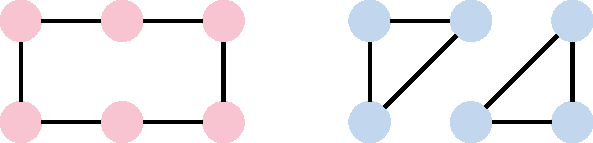
\includegraphics[width=\linewidth]{figures/tikz_WL.pdf} 一个简单例子：WL 检验无法区分\emph{六元环}与\emph{两个三角形}。}而且有许多它无法区分非同构图的简单例子，但其表达能力最终与 GNN 紧密相关。\citet{morris2019weisfeiler} 和 \citet{xu2018powerful} 的分析都得出了一个惊人的结论：符合第 \ref{sec:gnn-intro} 节所述三种类型之一的\emph{任何} GNN，其能力都不可能超过 WL 检验！

要准确达到这一表示能力水平，必须对 GNN 更新规则施加某些约束。\citet{xu2018powerful} 表明，在离散特征域中，GNN 使用的聚合函数必须是\emph{单射的}，而\emph{求和}是一个关键代表。\marginnote{最大化和平均等常见聚合器在这一点上有所不足，因为它们无法区分例如邻居多重集 $\ldblbrace \vec{a}, \vec{b}\rdblbrace$ 与 $\ldblbrace \vec{a}, \vec{a}, \vec{b}, \vec{b}\rdblbrace$。}根据分析结果，\citet{xu2018powerful} 提出了 Graph Isomorphism Network（GIN）；它是该框架下具有最大表达能力的一个简单而强大的 GNN 实例，也可以用我们提出的卷积 GNN 类型表达。

最后值得注意的是，这些发现不能推广到\emph{连续}节点特征空间。事实上，\citet{corso2020principal} 利用 Borsuk--Ulam 定理 \citep{borsuk1933drei} 证明，在假定节点特征为实值时，得到单射聚合函数需要\emph{多个}聚合器（具体而言，其数量等于接收节点的\emph{度}）。\marginnote{这类聚合器的一个例子是邻居多重集的\emph{矩}。}他们的发现推动了 Principal Neighbourhood Aggregation（PNA）架构；该架构提出了一个经验上强大且稳定的多聚合器 GNN。

\paragraph{高阶方法} % and Topological Data Analysis}

前几段的发现并不否定 GNN 的实际效用。事实上，在许多现实应用中，输入特征足够\emph{丰富}，尽管存在上述限制，仍能支持对图结构进行有用的判别计算。\marginnote{相比之下，上述限制几乎总是针对\emph{无特征}或\emph{带类别特征}的图。}

不过，一个重要推论是，GNN 在检测图内某些基本\emph{结构}方面相对较弱。在 WL 检验的具体局限或失败案例引导下，多项工作提出了\emph{更强的} GNN 变体；可以\emph{证明}它们比 WL 检验更强，因此很可能适用于需要这类结构检测的任务。\marginnote{一个突出实例是计算化学：分子图中是否存在芳香\emph{环}，可能强烈影响分子的化学功能。}

寻找表达能力更强的 GNN，最直接的地方或许就是 WL 检验本身。事实上，可以考虑 WL 检验的\emph{层次体系}来增强原始 WL 检验，使 $k$-WL 检验为节点的 $k$\emph{-元组}赋予表示 \citep{morris2017glocalized}。\citet{morris2019weisfeiler} 把 $k$-WL 检验直接转化为\emph{高阶} $k$-GNN 架构；\marginnote{已有一些工作采用 $\delta$-$k$-LGNN \citep{morris2020weisfeiler} 等方法，尝试稀疏化 $k$-GNN 的计算。}可以证明，该架构比此前考虑的 GNN 类型更强。然而，它必须维护元组表示，这意味着实践中很难扩展到 $k=3$ 以上。

与此同时，\citet{maron2018invariant,maron2019provably} 研究了节点 $k$-元组上的不变与等变图网络的刻画。他们不仅证明了一个令人惊讶的结果——\emph{任意}不变或等变图网络都可以表示为有限个生成元的线性组合，而生成元数量仅依赖于 $k$——还证明了这类层的表达能力等价于 $k$-WL 检验，并提出一种经验上可扩展且可证明具有 3-WL 能力的变体。

除了推广计算表示的域之外，大量工作还用于分析 1-WL 的具体失败案例，并扩充 GNN 的\emph{输入}，以帮助模型区分这些情形。一个常见例子是为节点附加\emph{标识特征}，这有助于检测结构。\marginnote{例如，如果一个节点在 $k$ 跳之外看到自己的标识符，就直接说明它位于一个 $k$-环内。}相关方案包括 \emph{one-hot} 表示 \citep{murphy2019relational}，以及纯\emph{随机}特征 \citep{sato2020random}。

更广泛地说，已有许多工作尝试在消息传递过程中纳入\emph{结构}信息，或者调节消息函数，或者调节承载计算的图。\marginnote{在计算化学领域，人们常假定分子功能由子结构（即\emph{官能团}）驱动；这直接启发了在\emph{基元}层面对分子建模。相关参考文献见 \cite{jin2018junction,jin2020hierarchical,fey2020hierarchical}。}其中一些有趣的研究方向包括采样\emph{锚节点集合} \citep{you2019position}、基于\emph{Laplacian 特征向量}聚合 \citep{stachenfeld2020graph,beaini2020directional,dwivedi2020generalization}，以及执行\emph{拓扑数据分析}，将其用于位置嵌入 \citep{bouritsas2020improving} 或驱动消息传递 \citep{bodnar2021weisfeiler}。

 
% Lastly, it is important to note that one of the most popularised and impactful applications of graph representation learning at the time of writing this book exactly corresponds to using GNNs to accurately screen potential drugs, leading to discovery of a novel potent antibiotic, Halicin \citep{stokes2020deep}. 

%\michael{
\paragraph{信号处理与调和分析}
自卷积神经网络早期取得成功以来，研究者便借助调和分析、图像处理和计算神经科学中的工具，尝试提供一个能够解释其效率的理论框架。
$M$-理论是一个受视觉皮层启发的框架，由 Tomaso Poggio 及其合作者 \citep{riesenhuber1999hierarchical, serre2007feedforward} 开创，基于可在某些对称群下操纵的模板概念。计算神经科学中产生的另一个重要模型是\emph{可转向金字塔}；它由 \cite{simoncelli1995steerable} 提出，是一种对某些输入变换具有良好性质的多尺度小波分解。可转向金字塔是早期纹理生成模型 \citep{portilla2000parametric} 的核心元素；随后，人们用深度 CNN 特征取代可转向小波特征，改进了这些模型 \cite{gatys2015texture}。
最后，由 St{\'e}phane \cite{mallat2012group} 引入、并由 \cite{bruna2013invariant} 发展的散射变换，通过用多尺度小波分解取代可训练滤波器，为理解 CNN 提供了一个框架，同时展示了形变稳定性以及深度在架构中的作用。


% Wavelets Mallat

% Multiscale analysis

% Simoncelli

% Poggio
%}


%[spectral]

\paragraph{图与网格曲面上的信号处理}
另一类重要的图神经网络通常称为\emph{谱方法}；它源于本文一位作者的工作 \citep{bruna2013spectral}，并采用\emph{图 Fourier 变换}这一概念。
%
这一构造源自信号处理与计算调和分析研究群体；在 2000 年代末和 2010 年代初，处理非 Euclidean 信号在这些领域中日益受到重视。Pierre Vandergheynst 团队 \citep{shuman2013emerging} 和 Jos{\'e} Moura 团队 \citep{sandryhaila2013discrete} 的有影响力论文普及了“图信号处理”（GSP）概念，以及基于图邻接矩阵与 Laplacian 矩阵特征向量的 Fourier 变换推广。
%
\citet{defferrard2016convolutional} 和 \cite{kipf2016semi} 提出的依赖谱滤波器的图卷积神经网络，是该领域被引用最多的工作之一，也很可能重新点燃了近年来人们对图上机器学习的兴趣。


值得注意的是，在计算机图形学与几何处理领域，非 Euclidean 调和分析比图信号处理至少早十年。流形与网格曲面上的谱滤波器可以追溯到 \cite{taubin1996optimal} 的工作。进入 2000 年代后，随着%Zachi Karni and Craig Gotsman
\cite{karni2000spectral} 关于谱几何压缩的有影响力论文，以及 \cite{levy2006laplace} 关于把 Laplacian 特征向量用作非 Euclidean Fourier 基的工作，这些方法进入主流。
%
谱方法已被用于多种应用，\marginnote{Roee Litman 和 Alex Bronstein（\citeyear{litman2013learning}）提出了与谱图 CNN 类似的可学习形状描述符；后者是本文一位作者的孪生兄弟。}其中最突出的是构造形状描述符 \citep{sun2009concise} 和函数映射 \citep{ovsjanikov2012functional}；在本文写作时，这些方法仍广泛用于计算机图形学。


%\michael{Kova\v{c}evi\'{c}}




\paragraph{计算机图形学与几何处理}
%\michael{Metric models, isometry-invariance, symmetry}
计算机图形学与几何处理领域的多位作者提出了基于内蕴度量不变量的形状分析模型 \citep{elad2003bending,memoli2005theoretical,bronstein2006generalized}；本文一位作者在其早期著作中对此作了深入讨论 \citep{bronstein2008numerical}。同一领域还研究了内蕴对称性的概念 \cite{raviv2007symmetries,ovsjanikov2008global}。
%
首个网格曲面深度学习架构 Geodesic CNN，由本文一位作者所在的团队开发 \citep{masci2015geodesic}。该模型使用具有共享权重的局部滤波器，并将其应用于沿测地线定义的径向斑块。它是本文另一位作者后来开发的规范等变 CNN \citep{cohen2019gauge} 的一种特殊设置。
%
同一团队的 Federico \cite{monti2017geometric} 提出了 Geodesic CNN 的推广 MoNet，采用可学习的聚合运算。MoNet 在网格曲面的局部结构特征上使用类似注意力的机制，并已被证明同样适用于一般图。
%
图注意力网络（GAT）由本文另一位作者提出 \citep{velickovic2018graph}；从技术上说，它可以视为 MoNet 的一个特殊实例。GAT 把 MoNet 的注意力机制推广到同时纳入节点特征信息，从而突破了先前工作中相关性纯粹源于结构的限制。它是目前最流行的 GNN 架构之一。


在计算机图形学背景下，还值得一提的是，集合上学习的思想 \citep{zaheer2017deep} 同时也由 Stanford 的 Leo Guibas 团队以 PointNet 之名发展，用于分析 3D 点云 \citep{qi2017pointnet}。该架构催生了多项后续工作，其中包括本文一位作者提出的 Dynamic Graph CNN（DGCNN，\cite{wang2019dynamic}）。DGCNN 使用最近邻图捕获点云的局部结构，使信息能够在节点之间交换；该架构的关键特征是即时构造图，并根据下游任务在神经网络各层之间更新图。
%
后一项性质使 DGCNN 成为“潜在图学习”最早的实现形式之一，而这一方向随后得到了大量后续研究。对 DGCNN 的 $k$ 最近邻图方案的推广，包括通过双层优化 \citep{franceschi2019learning}、强化学习 \citep{kazi2020differentiable} 或直接监督 \citep{velivckovic2020pointer}，更明确地控制这些图的边。与此独立地，NRI 模型 \citep{kipf2018neural} 开启了一个变分方向，即从计算得到的\emph{后验}分布中以概率方式采样边。尽管它仍依赖关于节点数的二次计算，却能显式编码所选边的不确定性。
%\michael{Mention algorithmic reasoning and Cranmer's work on symbolic equations?}

在没有给定图的情况下进行图上学习，另一个非常流行的方向是在\emph{完全图}上执行 GNN 式计算，让网络自行推断利用连通性的方式。这一需求在自然语言处理中尤为突出，因为句子中的不同词语以高度非平凡且非顺序的方式相互作用。在词语完全图上进行运算，促成了 Transformer 模型的最初实现 \citep{vaswani2017attention}；它取代循环模型和卷积模型，成为神经机器翻译的最先进方法，并掀起了跨越 NLP 与其他领域边界的大量相关工作。全连接 GNN 计算也同时出现在仿真 \citep{battaglia2016interaction}、推理 \citep{santoro2017simple} 和多智能体 \citep{hoshen2017vain} 应用中；当节点数相对较小时，它至今仍是一种流行选择。
%
%Most recent works 

%manifold learning 

%Rotation-equivariant CNNs

\paragraph{算法推理}
在本节的大部分讨论中，我们给出的例子都是由\emph{空间}诱导的几何，它们进而塑造底层域及其不变性与对称性。然而，在\emph{计算}设置中同样存在大量不变性与对称性实例。它与几何深度学习许多常见设置的一项关键区别在于，链接不再需要编码任何相似性、接近程度或关系类型；它们只规定所连接数据点之间数据流的“配方”。

神经网络的计算转而模仿\emph{算法}的推理过程 \citep{cormen2009introduction}，而算法的控制流与中间结果还会诱导出额外的不变性。\marginnote{例如，Bellman--Ford 寻路算法 \citep{bellman1958routing} 的一个不变量是：在 $k$ 步之后，它总能计算出使用不超过 $k$ 条边到达源节点的最短路径。}在算法领域，对输入假定的不变量常称为\emph{前置条件}，而算法所保持的不变量称为\emph{后置条件}。

同名研究方向\emph{算法推理} \citep[Section 3.3.]{cappart2021combinatorial} 旨在构造能够适当保持算法不变量的神经网络架构。该领域研究了通用神经计算机的构造，例如 \emph{neural Turing machine} \citep{graves2014neural} 和 \emph{differentiable neural computer} \citep{graves2016hybrid}。尽管这类架构具备通用计算的所有特征，但它们一次引入多个组件，因而往往难以优化；实践中，\citet{santoro2017simple,santoro2018relational} 所提出的简单关系推理器几乎总能超过它们。

由于建模复杂后置条件颇具挑战性，关于学习执行的归纳偏置研究 \citep{zaremba2014learning} 大多聚焦于基本算法（例如简单算术）。该领域的突出实例包括 \emph{neural GPU} \citep{kaiser2015neural}、\emph{neural RAM} \citep{kurach2015neural}、\emph{neural programmer-interpreters} \citep{reed2015neural}、\emph{neural arithmetic-logic units} \citep{trask2018neural,madsen2020neural} 和 \emph{neural execution engines} \citep{yan2020neural}。

GNN 架构的快速发展使模拟具有\emph{超线性}复杂度的组合算法成为可能。\citet{xu2019can} 开创的\emph{算法对齐}框架从理论上证明，GNN 与动态规划\emph{对齐} \citep{bellman1966dynamic}，而大多数算法都可以用动态规划这种语言表达。与此同时，本文一位作者从经验上表明，实践中可以设计并训练与算法不变量对齐的 GNN \citep{velivckovic2019neural}。随后，人们实现了与\emph{迭代算法} \citep{tang2020towards}、\emph{线性对数算法} \citep{freivalds2019neural}、\emph{数据结构} \citep{velivckovic2020pointer} 和\emph{持久内存} \citep{strathmann2021persistent} 的对齐。这类模型还在\emph{隐式规划器} \citep{deac2020xlvin} 中得到实际应用，进入了\emph{强化学习}算法领域。

与此同时，使用 GNN 进行\emph{物理仿真}也取得了显著进展 \citep{sanchez2020learning,pfaff2020learning}。这一方向对可泛化 GNN 的设计给出了许多相同建议。这种对应关系并不意外：算法可以表述为离散时间仿真，而仿真通常实现为逐步算法，因此两个方向都需要保持相似类型的不变量。

与算法推理研究紧密相连的是对\emph{外推}的度量。外推是神经网络一个众所周知的痛点，因为多数成功案例都发生在\emph{分布内}泛化时，即训练数据中的模式能够恰当地预示测试数据中的模式。然而，无论输入的大小或生成分布如何，算法不变量都必须得到保持；这意味着训练集很可能无法覆盖实践中遇到的所有可能场景。\citet{xu2020neural} 从几何角度论证了由整流激活支持的外推 GNN 需要满足什么条件：其组件和特征化方式必须经过设计，使组成模块（例如消息函数）只学习\emph{线性}目标函数。\citet{bevilacqua2021size} 提出从\emph{因果推理}视角考察外推，从而得到图的\emph{环境不变}表示。

\paragraph{几何深度学习}
最后的历史评述涉及本文的名称本身。
%
术语“几何深度学习”最早由本文一位作者在其 2015 年 ERC 资助申请中提出，并经 IEEE Signal Processing Magazine 上的同名论文 \citep{bronstein2017geometric} 得到普及。该论文虽然“带着几分谨慎”，却宣称出现了“一个新领域正在诞生”的迹象。鉴于图神经网络近来的流行、不变性与等变性观念在广泛机器学习应用中日益得到采用，以及我们正在撰写本文这一事实，或许可以认为这一预言至少部分实现了。
%
名称“4G: Grids, Graphs, Groups, and Gauges”由 Max Welling 为 ELLIS 几何深度学习项目创造；该项目由本文的两位作者共同主持。必须承认，最后一个“G”多少有些牵强，因为底层结构是流形与丛，而不是规范。
%
在本文中，我们又加入了一个“G”，即 Geodesics，用来指代流形的度量不变量与内蕴对称性。


%{\footnotesize
